\section{作品概述}

\subsection{功能与特性}
本作品基于安路 HX4S20C 开发板（主芯片 EG4S20BG256），是一台集图片展示、音乐播放和动态数字艺术于一体的多媒体交互画框。上电后，系统自动查找 TF 卡根目录中的图片与音乐，经 FPGA 解析、缩放、缓存与图层合成，由 HDMI 同时输出 720p 画面和 48 kHz 立体声；观众用板载按键和拨码开关切图、选曲、调节画面和进入动态场景。

作品完成了赛题的基础要求与五类拓展功能 [1,2]，全部功能集成在同一固化镜像中，上电即可运行：
\begin{itemize}
\item 基础功能：TF 卡 BMP 图片读取与 HDMI 显示；按键手动切图与可配置周期的自动轮播；48 kHz 音频经 HDMI 播放；镜像固化至配置 Flash，上电自启动。
\item 拓展功能：中文滚动字幕叠加；淡出—黑场—淡入切图转场；不同尺寸图片的等比双线性缩放；亮度、对比度、音量等参数的中文菜单实时调节；基于真实 PCM 样本的音频可视化。
\item 特色功能：四季动态夜城，以同一座城市呈现四种季节与天气，画面由 FPGA 实时生成，并随背景音乐联动。
\end{itemize}

四季动态夜城是作品的核心展示内容。雨夜霓虹、黄昏雷云、薄雾深夜和飘雪清晨共用同一座城市，色彩、天气和灯光的变化形成四种持续运动的画面；街区广告屏随正在播放的音乐跳动，退出动态模式后直接回到原来的静态图片。图\ref{fig:seasons}展示四种场景的设计效果。

\begin{figure}[H]
\centering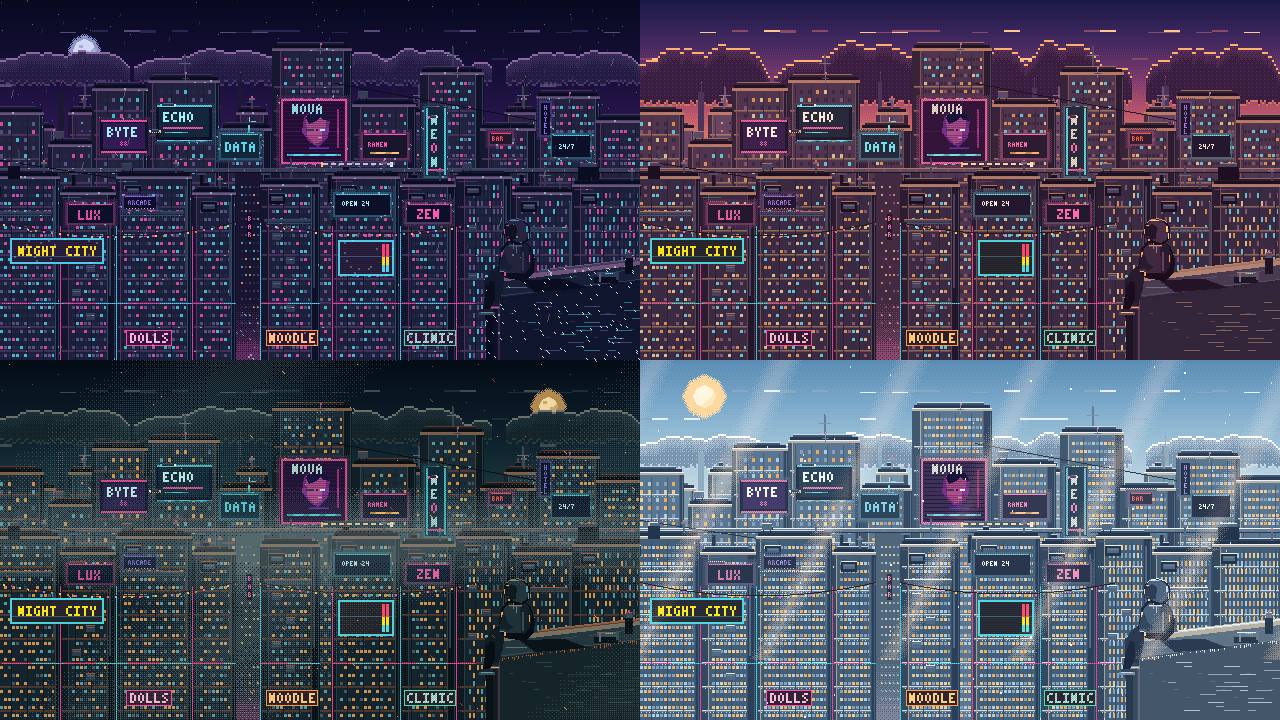
\includegraphics[width=0.96\textwidth]{figures/four_seasons_design.png}
\caption{四季动态夜城设计效果}\label{fig:seasons}
\end{figure}

\subsection{应用领域}
作品面向需要长期、离线展示音画内容的场合：
\begin{itemize}
\item \textbf{展厅与博物馆}：静态图片承担展品介绍与科普讲解，中文字幕补充说明，背景音乐营造氛围；
\item \textbf{商业空间与橱窗}：轮播产品图片，空闲时切换到动态夜城作为吸引视线的数字艺术背景；
\item \textbf{校园与公共信息屏}：轮播通知、安全提示等图片，内容更新只需替换 TF 卡素材；
\item \textbf{家居数字画框}：播放个人照片与音乐，四季场景提供随时间变化的装饰画面。
\end{itemize}
设备不依赖网络和上位机，准备好素材后由开发板独立运行；更换内容只需替换 TF 卡中的文件。

\subsection{主要技术特点}
\textbf{1. 纯 FPGA 实现的完整音画系统。}FAT32 根目录查找、BMP 与 WAV 解析、图像缩放、SDRAM 帧缓存、图层合成、音量处理和 HDMI 音视频封装全部由 FPGA 硬件逻辑完成，不使用软核处理器或外部主控。

\textbf{2. 多时钟域并行流水架构。}4 个 PLL 产生 50 MHz 卡访问、40 MHz 存储、25 MHz 画面合成、74.25 MHz 像素时钟及其 5 倍频串行时钟。各域以异步 FIFO、翻转令牌和请求／应答握手衔接，读卡、写缓存、扫描输出和音频播放并行推进、互不阻塞。

\textbf{3. 动态画面实时生成。}动态场景由像素坐标、季节色板和帧计数实时计算，不占用 TF 卡读取带宽；字幕、菜单、音频柱作为独立图层按坐标叠加，无需额外帧缓存。

\textbf{4. 资源高度集成。}在 19600 LUT 的器件中同时容纳基础功能、五类扩展和动态场景，LUT 利用率 91\%，32 Kb RAM 块与 PLL 全部用满，全部时钟域时序收敛。

\subsection{主要性能指标}
\begin{center}\small
\begin{tabular}{p{4.0cm}>{\raggedright\arraybackslash}p{9.5cm}}
\toprule
项目 & 指标\\\midrule
处理平台 & HX4S20C；EG4S20BG256；板载 50 MHz 时钟\\
视频输出 & HDMI，$1280\times720$@60 Hz，像素时钟 74.25 MHz；内部合成画布 $640\times360$\\
音频输出 & 48 kHz、16 位、双声道 PCM WAV，经 HDMI 传输；配套素材四首曲目可在菜单中选择\\
图片输入 & 24 位非压缩 BMP，根目录最多六张，宽高不超过 $1920\times1080$，运行时等比适配\\
图片缓存 & SDRAM 六帧缓存，共 5.27 MiB，切图无需重新读卡\\
自动轮播 & \tablegroup{3 / 5 / 15} 秒三档可选\\
动态场景 & 四季四景，1012 个城市图块，40 组季节色板，逐像素实时生成\\
交互与扩展 & 中文菜单、滚动字幕、淡入淡出转场、\tablegroup{亮度 / 对比度 / 音量}调节、64 柱幅度历史与街区音乐屏\\
资源占用 & LUT \tablegroup{17884 / 19600}（91\%）；SLICE \tablegroup{9192 / 9800}；PLL \tablegroup{4 / 4}\\
时序结果 & 全部时钟域 setup 与 hold 余量均为正，setup 最差余量 $+0.357$ ns，无时序违例\\
\bottomrule
\end{tabular}
\end{center}

\subsection{主要创新点}
\textbf{1. 一城四季的实时数字艺术。}作品没有把动画做成视频文件，而是把城市拆分为 $8\times8$ 像素图块，由 FPGA 按坐标查表并叠加实时天气与灯光。1012 个去重图块按实际颜色数分级编码：143 个只需 1 bit／像素，369 个使用 2 bit／像素，其余 500 个使用 4 bit／像素，比全部采用 4 bit 编码节省约 29\% 的图块存储。整座城市的图块与映射数据合计约 0.24 Mbit，而四张 $640\times360$ 真彩静图需要约 22.1 Mbit，相差 90 倍以上；若以 30 帧／秒视频播放同等画面，10 秒即需约 1.66 Gbit。实时生成使四季场景在不占用读卡带宽的情况下持续运动。

\textbf{2. 真实音频驱动的双层视觉反馈。}主画面 64 柱幅度历史和夜城街区广告屏的 12 柱音乐屏都直接取自播放链路中经音量处理后的 PCM 样本。作品展示随时间滚动的幅度包络，没有采用频谱：观众不需要音频知识，就能看到鼓点和旋律起伏与柱形同步跳动；调节音量时，声音与柱高一起变化。幅度计算只需累加与移位，节省出的乘法器和存储资源用于实现动态场景。

\textbf{3. 完整帧呈现的多媒体融合。}六帧 SDRAM 缓存、运行时等比缩放、淡入淡出转场、中文菜单与滚动字幕协同工作；切图时只有完整写入的画面才会被发布显示，HDMI 扫描和音乐播放全程不中断。静图展示与动态场景共用同一套音画输出和交互控制，切换模式时只改变显示内容，不需要重新加载系统。

\subsection{设计流程}
设计按“基础链路优先、功能逐级集成”的原则推进：首先完成需求分解与板卡接口确认，建立 TF 读图、SDRAM 缓存和 HDMI 音画输出的基础链路；随后在统一的时钟与资源预算内逐步加入缩放、六帧缓存、图层、字幕、菜单和动态场景；每项功能经模块仿真、布局布线和上板验证后再进入下一轮集成，最终以同一镜像固化并验证上电自启动。图\ref{fig:workflow}概括该过程。

\begin{figure}[H]\centering
\begin{tikzpicture}[node distance=7mm, box/.style={draw,rounded corners,align=center,minimum width=2.7cm,minimum height=0.8cm,fill=blue!5}, arr/.style={-{Latex},thick}]
\node[box] (a) {需求与接口}; \node[box,right=of a] (b) {音画基础链路}; \node[box,right=of b] (c) {缓存与图层};
\node[box,below=of c] (d) {动态场景与交互}; \node[box,left=of d] (e) {仿真与布局布线}; \node[box,left=of e] (f) {固化与实物验证};
\draw[arr](a)--(b); \draw[arr](b)--(c); \draw[arr](c)--(d); \draw[arr](d)--(e); \draw[arr](e)--(f);
\draw[arr,dashed](e.south)--++(0,-0.45)-|node[pos=0.25,below,font=\small]{迭代优化}(d.south);
\end{tikzpicture}
\caption{作品设计与验证流程}\label{fig:workflow}
\end{figure}
